%\chapter{Empirical Work}


\chapter{Interviews with Working Professionals}

\chapter{Definition of Solution Objectives}

\chapter{Prototype Design and Development}

\chapter{Proof-of-Concept Demonstration}













%
%\section{Instruction included in the original FHBgld word processor template}
%Die Durchführung der empirischen Untersuchung ist nachvollziehbar zu dokumentieren sowie auch die dabei aufgetretenen Probleme und deren Behandlung. Der Umfang ergibt sich aus der Art der Bearbeitung.  
%
%Tabelle 1 zeigt ein Bespiel für eine Tabelle. 
%
%\begin{figure}[ht]
%	\centering
%	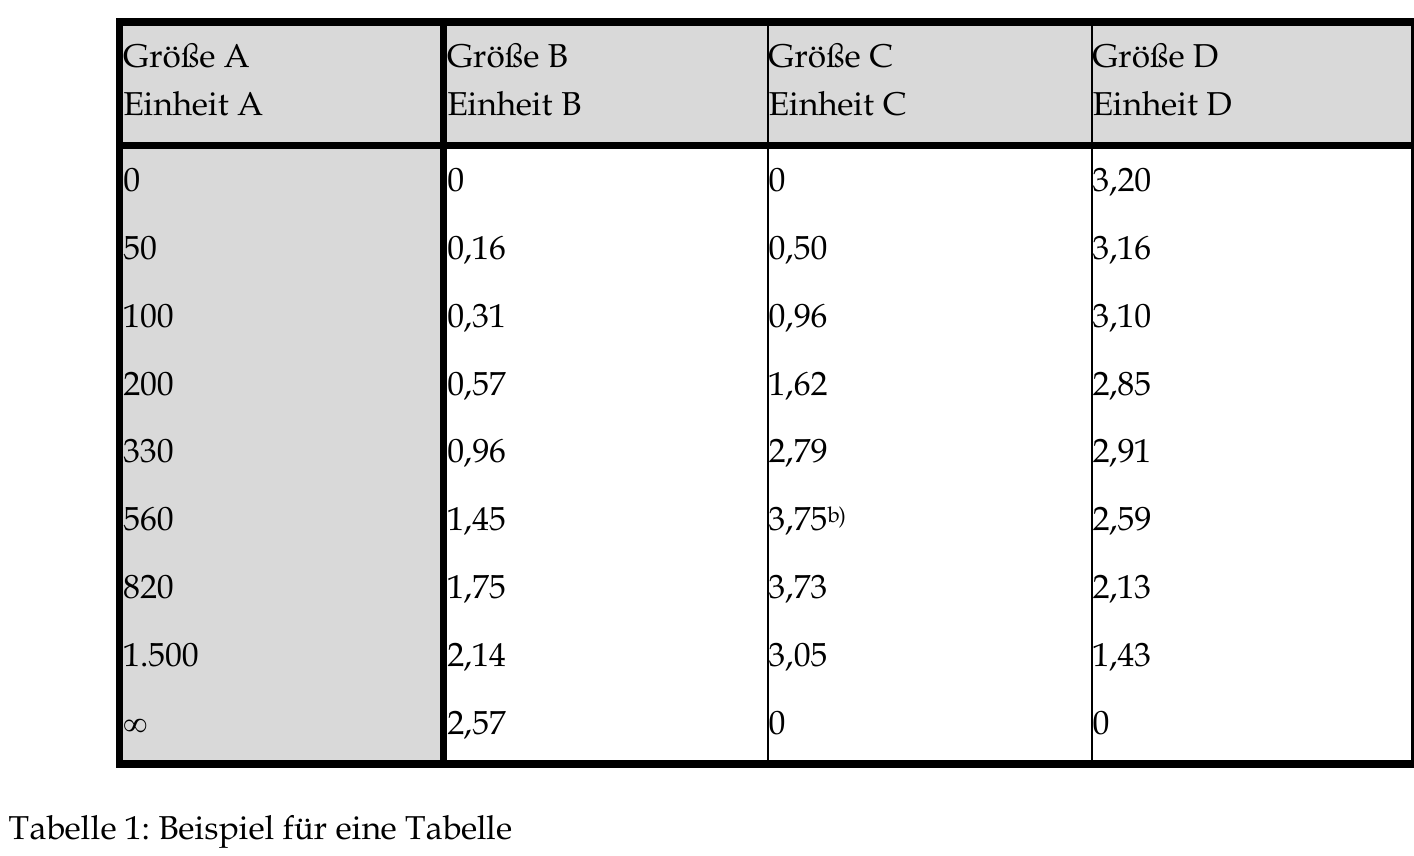
\includegraphics[width=0.7\linewidth]{figures/Word_Table}
%	\caption{Screenshot example from FHBgld word processor template}
%	\label{fig:wordtable}
%\end{figure}
%Abbildung 1 zeigt ein Beispiel für eine Abbildung oder Grafik.
%\begin{figure}
%	\centering
%	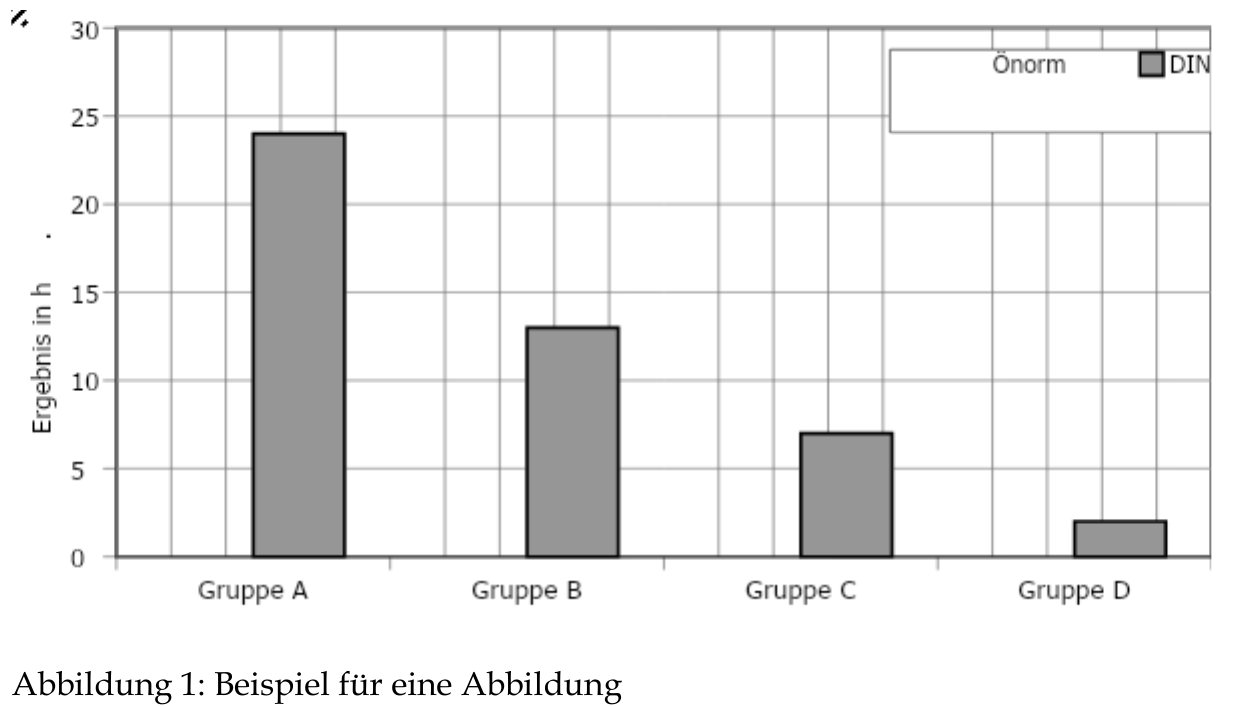
\includegraphics[width=0.7\linewidth]{figures/Word_Diagram}
%	\caption{Screenshot example from FHBgld word processor template}
%	\label{fig:worddiagram}
%\end{figure}
%\linebreak
%Mathematisch werden die Zusammenhänge wie im Figure \ref{fig:wordformel} beschrieben.
%\begin{figure}
%	\centering
%	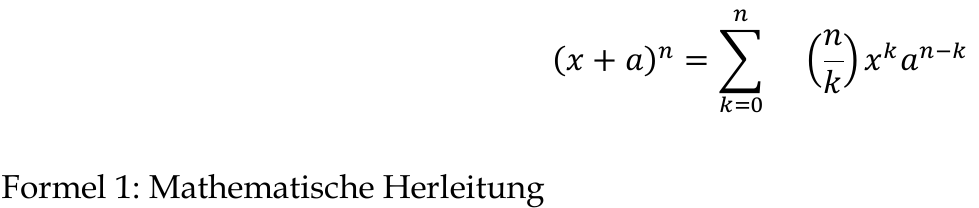
\includegraphics[width=0.7\linewidth]{figures/Word_Formel}
%	\caption{Screenshot example from FHBgld word processor template}
%	\label{fig:wordformel}
%\end{figure}
%
%\section{Tables and Images with \LaTeX}
%One of the great advantages of \LaTeX{} is that all it needs to know is
%the structure of a document, and then it will take care of the layout
%and presentation itself.  So, here we shall begin looking at how exactly
%you tell \LaTeX{} what it needs to know about your document.
%
%\subsection{Tables}
%In this sub-section, a simple table is inserted. To add reference to the table, see (cf. Table~\hyperref[tab:tableexample0]{\ref{tab:tableexample0}}):
%
%%A simple table.  The center environment is first set up, otherwise the
%%table is left aligned.  The tabular environment is what tells Latex
%%that the data within is data for the table.
%% https://en.wikibooks.org/wiki/LaTeX/Tables
%\begin{table}[htb]
%	\begin{tabular}{|b{7cm}|c|}
%		%The tabular environment is what tells Latex that the data within is
%		%data for the table.  The arguments say that there will be two
%		%columns, both left justified (indicated by the 'l', you could also
%		%have 'c' or 'r'.  The bars '|' indicate vertical lines throughout
%		%the table.
%		
%		\hline  % Print horizontal line
%		\fontsize{11pt}{12pt}\selectfont Command & Level \\ \hline  % Columns are delimited by '&'.  And
%		%rows are delimited by '\\'
%		\fontsize{10pt}{14pt}\selectfont Some sections to provide some examples: & \\
%		\texttt{\textbackslash part\{\emph{part}\}} & -1 \\
%		\texttt{\textbackslash chapter\{\emph{chapter}\}} & 0 \\
%		\texttt{\textbackslash section\{\emph{section}\}} & 1 \\
%		\texttt{\textbackslash subsection\{\emph{subsection}\}} & 2 \\
%		\texttt{\textbackslash subsubsection\{\emph{subsubsection}\}} & 3 \\
%		\texttt{\textbackslash paragraph\{\emph{paragraph}\}} & 4 \\
%		\texttt{\textbackslash subparagraph\{\emph{subparagraph}\}} & 5 \\
%		\hline
%		
%	\end{tabular}
%	\caption{some description of the table}
%	\label{tab:tableexample0}
%\end{table}
%
%\subsubsection{More tabular examples}
%
%First, a plain simple example for a FHBgld table, see table~\hyperref[tab:tab:tableexample1]{\ref{tab:tableexample1}}.
%
%\begin{table}[h]
%	\centering
%	\begin{tabular}{|b{1cm}|b{2cm}|b{3cm}|b{4cm}|}
%		\hline
%		\multicolumn{4}{|l|}{\fontsize{11pt}{12pt}\selectfont\noindent First line in 11pt fontsize } \\ \hline
%		1cm & 2cm & 3cm & 4cm \\ \hline
%		from & here on & the table & font size \\ \hline
%		will & be as & defined & in class, that is 10pt\footnote{yes, really!} \\ \hline
%		will & be as & defined & in class, that is 10pt\footnote{yes, really!} \\ \hline
%		will & be as & defined & in class, that is 10pt\footnote{yes, really!} \\ \hline
%		will & be as & defined & in class, that is 10pt\footnote{yes, really!} \\ \hline
%		will & be as & defined & in class, that is 10pt\footnote{yes, really!} \\ \hline
%	\end{tabular}
%	\caption{some description of the table}
%\label{tab:tableexample1}
%\end{table}
%
%Next, a table with nine columns, see table~\hyperref[tab:tableexample2]{\ref{tab:tableexample2}}.
%
%\begin{table}[h]
%	\centering
%	\begin{tabular}{|*{9}{l|}}
%		\hline
%		{\fontsize{11pt}{12pt}\selectfont This} & {\fontsize{11pt}{12pt}\selectfont table} & {\fontsize{11pt}{12pt}\selectfont has} & {\fontsize{11pt}{12pt}\selectfont way} & {\fontsize{11pt}{12pt}\selectfont too } & {\fontsize{11pt}{12pt}\selectfont many} & {\fontsize{11pt}{12pt}\selectfont columns}, & {\fontsize{11pt}{12pt}\selectfont does'nt} & {\fontsize{11pt}{12pt}\selectfont it?} \\ \hline
%		One & Two & Three & Four & Five & Six & Seven & Eight & Nine! \\ \hline
%		At & least & the & first & column & has & 11pt & font & size. \\ \hline
%	\end{tabular}
%	\caption{some description of the table}
%	\label{tab:tableexample2}
%\end{table}
%
%\subsection{Images}
%% Here is how to insert an image as a figure. There is a lot more you can do
%% when inserting images, check out: https://en.wikibooks.org/wiki/LaTeX/Importing_Graphics
%
%\begin{figure}[h]
%	\centering
%	
\includegraphics[width=0.3\textwidth]{figures/logo_nontransparent.jpg}
%	\caption{Image Example}
%	\label{fig:image_example}
%\end{figure}
%
%When an image is inserted, you can refer to it like this (cf. Figure~\hyperref[fig:image_example]{\ref{fig:image_example}}).
%
%\subsubsection{A Subsubsection}
%As one last example, this is how you can insert a sub-sub-section! Have fun
%writing your thesis with \LaTeX{}!
%
%\lipsum[2-3]
%\raggedbottom
%
%\pagebreak
